\documentclass[10pt]{article}
\usepackage[a4paper,margin=19mm]{geometry}
\usepackage{graphicx,booktabs,hyperref}
\usepackage[T1]{fontenc}
\setlength{\parindent}{0pt}
\setlength{\parskip}{6pt}
\begin{document}
{\Large Bounded-memory Boolean Macaulay passes}\par
Execution record, 18 October 2026. Items 7 and 9; public synthetic inputs.

Eight degree-4 passes on actual chained S3 Weil-descended systems completed.
Four small controls agreed exactly with an independent dense bit-matrix RREF.
The larger passes remain independently unverified. This is a fixed-degree
row-reduction result, not full F4, iterative closure, solving degree, or an
ECDLP cost result.

\begin{center}
\begin{tabular}{rrrrl}\toprule
$n$ & $\ell$ & Variables & Rows / rank & Dense RREF control\\\midrule
5&2&18&1,050 / 987&Exact equality, both policies\\
9&3&30&4,752 / 4,648&Exact equality, both policies\\
15&5&50&20,670 / 20,490&256 MiB reference limit refused\\
17&6&58&31,110 / 30,888&Open on diagnostic continuation\\\bottomrule
\end{tabular}
\end{center}
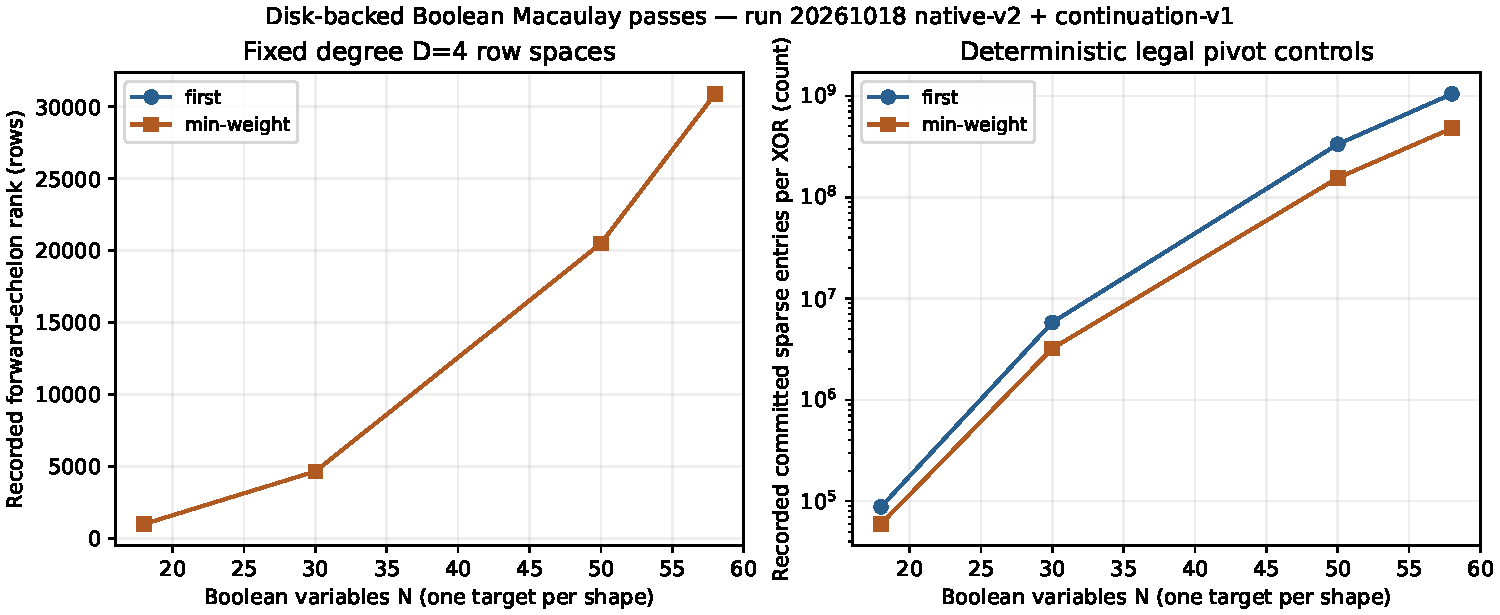
\includegraphics[width=\textwidth]{passes.pdf}

One target [17]G per shape and policy; $K_1$ curves over $\mathbf F_{2^n}$,
polynomial-basis subspaces, $m=4$, $D=4$. Graph values are native recorded
counters. Large-case ranks are engine observations, not independent
certificates. Sparse-entry counters cover committed checkpoint history and
exclude rolled-back suffix work; they establish no full-cost speed comparison.

The n=5 zero-cache and row-31 checkpoint/restart controls returned the same
independently certified RREF. One hundred seeded native arithmetic/oracle
controls passed. Truncated streams, inadequate output disk, restart input SHA
mismatch, and the n=19/ell=7 layout requiring 66 variables failed closed.
The current exporter is limited to 64-bit monomials.

The original native-v1 launches exited 127 because /usr/bin/time was unavailable;
no scientific binaries ran in that attempt. A native wait4 launcher replaced it
and enforced a 536,870,912-byte child address-space ceiling. Initial n=15 runs
reached EOF before the dense oracle's 256 MiB allocation guard refused them.
Initial n=17 runs reached their 64 MiB trace cap. Copies of checkpoints/journals
were continued in fresh directories, preserving original failures.

\newpage
{\large Scope, accounting and evidence}\par
The pivot cache has an explicit 1,048,576-byte row-payload limit with LRU eviction.
Index/LRU metadata and temporary rows add overhead; the process-wide address-space
limit bounds total address space. Journal and trace caps are 1 GiB and 64 MiB
per phase. Row-size guards allow 16 MiB of terms; temporary XOR vector
reservations may use 32 MiB before the guard. The reducer is serial and disk-backed.
There is no GPU, distributed executor, or incumbent-oracle integration.

Per-process CPU, wall time and peak RSS are recorded separately for every launch
in resources.json files. The host was shared (isolation tier 0). Initial n=15
first/minimum-weight runs recorded 26,932/27,048 KiB peak RSS. Build, export,
generation, failed attempts, verification, copied state and resumed reductions
are separate phases. Journal counters omit index reconstruction/input reads
and rolled-back suffix work; process resource records retain their executed
costs. No matched external engine or full pipeline/rho comparison was run.

The policy hooks allow only choosing between rows with the same leading
monomial. First-pivot and minimum-weight controls log lead, row index, incoming
and pivot weight, replacement action, and feature/decision timer counts.
No learned model, training/calibration/heldout split, charged training experiment,
learned column policy or heldout transfer result exists in this deliverable.

Checkpoints flush journal data before atomically renaming metadata, binding input
SHA256, policy, cache size, next input offset, journal boundary and counters.
The tests establish the stated process restart and input-identity checks;
power-loss/fsync durability and arbitrary journal-corruption handling remain open.

Item 7 remains partial: canonical frontier ell=6/7 and guess-count ell=8/9 closure
trials, full F4/MutantXL scheduling, certified large-case replay and distributed/GPU
kernels remain outstanding. The selected n=17/ell=6 cell is a diagnostic, not a
substitution for a canonical frozen frontier requirement. Item 9 has deterministic
legal hooks only. No solving-degree, deployed-security or fastest-engine claim
is made. Canonical leaderboard and solving-degree plots stay unchanged.

\textbf{Reproducible evidence.} The study directory is
\texttt{research/ideas\_execution\_20261018/bounded\_memory/}.
Frozen protocols precede their respective trial scripts. Runs native-v1,
native-v2 and large-continuation-v1 retain exact argv, UTC times, exits, raw
stderr, resources, input/source/binary/dependency digests, checkpoints and traces.
Input metadata binds field structure, target coordinates, subgroup order and
subspace basis. Gzip archives preserve raw record contents; SHA256 manifests
refer to their uncompressed basenames. Full observations and links are in
REPORT.md and README.md.

\textbf{Sources.} Pinned source base:
\texttt{e063d98475589d9aba7ae265a8cba830927e3156}, with root-agent library
build repairs. The ANF builder and row family are from
\texttt{src/cryptanalysis/koblitz\_groebner.rs}; the existing sparse control context
is \texttt{sparse\_macaulay.rs}. Full F4 semantics in \texttt{pq\_f4\_f2.rs} are
explicitly outside this standalone reducer. No library core is edited here.
\end{document}
